

\title{\huge{The ecology and evolution of movement in fluctuating landscapes}}
\author{{Pratik R Gupte}}
\date{January 2019}

{\parindent0pt
	
{\large{\textbf{\textsf{Supervised by}}} \\
\large{Prof. Franz J Weissing} \\
\large{Dr. Allert I Bijleveld} \\
\large{Prof. Ton Groothuis} \\
\large{Prof. Theunis Piersma}}

}

\begin{figure}[h!]
	
	
\includegraphics[width=200pt, height = 80pt]{logo_affils.eps}
	\caption{}
	\label{fig:logoaffils}
\end{figure}

\begin{document}

\newpage

{\parindent0pt

\textbf{© Pratik R Gupte}

\textbf{Modelling Adaptive Response Mechanisms Group},\\
Groningen Institute for Evolutionary Life Sciences,\\
University of Groningen.

\textbf{Bijleveld Lab},\\
Department of Coastal Systems,\\
Royal Netherlands Institute for Sea Research.

\textbf{Contact information}

Groningen Institute for Evolutionary Life Sciences\\
University of Groningen\\
Nijenborgh 7-5172.0583, 9747 AG Groningen\\
Netherlands\\
p.r.gupte@rug.nl

\textbf{Supervisors}

Prof. FJ Weissing\\
Dr. AI Bijleveld\\
Prof. AGG Groothuis\\
Prof. T Piersma

\textbf{Promotors}

FJ Weissing\\
AGG Groothuis

\textbf{Funding}

Adaptive Life Programme -- Groningen Institute for Evolutionary Life
Sciences\\
Short term causes and long term consequences of adaptations to
environmental change

\begin{figure}[h!]
	
	
\includegraphics[width=200pt, height = 80pt]{logo_affils.eps}
	
	\label{fig:logoaffils}
\end{figure}
}

\newpage

\tableofcontents

\newpage

%\linenumbers

\addtolength{\topskip}{0pt plus 10pt}

%add parindent again

\part*{Summary}\label{part:Summary}
\addcontentsline{toc}{part}{Summary}

\setlength{\parindent}{3ex}

The \textbf{\emph{movement of animals}} has always fascinated humans, but modern biology has only now come to actively study movement as the linchpin of many processes. As movement studies seek to unify phenomena across scales, they must also contend with the idea that there are \textbf{\emph{consistent individual differences}} within many animal populations. These differences, whose evolution, development, and maintenance are still under debate, are estimated to have population level consequences.
One system in which consistent individual differences have been identified is that of \textbf{\emph{red knots}} \emph{Calidris canutus}, which forage on intertidal mudflats and vary along an axis of exploratory behaviour. Knots' and other foragers' movement is often strongly influenced by which \textbf{\emph{spatio-temporal change}} in the often unpredictable resource landscape. This system inspires questions about how movement strategies evolve in such landscapes, how they affect the landscapes on which they evolve, as well as how the interaction of the two gives rise to emergent phenomena such as structured communities.

This essay, an introduction to my work over the next two years, is organised over the following parts: first, the \textbf{\emph{Introduction}} contains key concepts in the fields of \emph{Animal movement, Movement as personality}, and \emph{Modelling movement}.
The second section, \textbf{\emph{About this project}}, lays out the questions I want to investigate for my PhD.
The third section, \textbf{\emph{Towards a model of wader movement}}, explains the conceptual and practical aspects of the models and empirical methods I propose to implement towards the goals I set myself. Section four, \textbf{\emph{Timeframe}} outlines the activities I will undertake over the period 2018 -- 2022 in terms of research, personal academic training, co-supervision of students, and academic output, culminating in a thesis submission in May 2022, and a thesis defence provisionally in September 2022.

For my PhD, I will attempt to break new ground for the field of animal movement by examining the evolution of movement strategies, with a special focus on the evolution of consistency in fluctuating environments. First, using simple, abstract models, I will examine under which conditions of environmental spatial predictability and temporal change one can expect the evolution of distinct movement types. Second, I will examine the ecological consequences of consistency in movement behaviour in heterogeneous landscapes. Third, I will tailor the former models to investigate consistency in exploratory behaviour in my model system, the shorebirds known as red knots (\emph{Calidris canutus}). Fourth, and finally, I will examine whether red knots tracked in the wild show movement types, and thus test the predictions of theory.

\newpage

\part{Introduction}

\section{Animal movement}

Animal movement across spatio-temporal scales -- from seasonal migration, to breeding aggregations, to diurnal cycles -- have been an important field of human knowledge throughout recorded history, and likely long before.
Even in more modern times, the two most successful paradigms of the natural sciences' century of insight, evolution by natural selection \citep{darwin1858} and island biogeography \citep{macarthur2001}, rely at least in part on the movement of animals to make their point.
Explicit treatment of the subject began with theoretical developments on the movement of freely moving and ideally rational agents. This led to nearly simultaneous advances in the understanding of the distribution of foragers at the landscape scale \citep{fretwell1970}, and the topology of groups of selfish agents \citep{hamilton1971}.
Theory on population spatial distributions soon incorporated fine-scale phenomena such as individual interactions and population structure, and was already a mature field with strong empirical support when reviewed by \citet{sutherland1996}.
Theoretical advances in the study of fine-scale movement itself, on the other hand, have lagged behind the measurement of the movement of individual animals \citep{holyoak2008}.

The recently emerged movement ecology paradigm \citep[MEP;][see Fig. 1]{nathan2008a} has sought to fill this gap, understanding ``movement itself as the focal theme\ldots{}by providing a unifying framework and common tools'' \citep{nathan2008}.
This paradigm urges practitioners to attempt to answer three questions: 1. \emph{Why} do organisms move? 2. \emph{Where} do organisms decide to move? 3. \emph{How} do organisms move?
This links (1) external stimuli, such as fear of predators \citep{laundre2001}, (2) sensory capacity, which translates into navigational ability and search strategies \citep[e.g.][]{bartumeus2008}, and (3) life-history dependent physiology and internal state \citep[eg.][]{fryxell2008}.
Movement ecology's rise has coincided with the beginning of ``a golden age of animal tracking science'' in the form of large-scale and high-resolution animal tracking \citep{hussey2015, kays2015}.
Biologging, i.e., the remote measurement of instantaneous organism state \citep{cooke2004}, and high-resolution animal tracking in particular, have led to remarkable insights into the detailed sub-units of movement behaviour, such as the energetics of predation and locomotion \citep[see e.g.][]{williams2004, scantlebury2014}.

\begin{figure}
    \includegraphics[width=0.7\linewidth]{fig02_nathan_etal_2008.png}
    \caption{The movement ecology paradigm places observed movement (\emph{path: U}) as both a consequence of prior factors, and a contributor to future ones. From Nathan et al. (2008).}
    \label{fig:fig02nathanetal2008}
\end{figure}

Despite advances in empirical methods, animal movement studies are still subject to limitations of scale. Among these are emergent group-size effects \citep{tunstrom2013}, which are difficult to quantify empirically notwithstanding recent advances \citep{handegard2012, kays2015, strandburg-peshkin2015a, dhanjal-adams2018}; a distinct problem when animal grouping is near-universal \citep{krause2002}.
The impracticality of research across scales of organisation (eg. physiology to population) has similarly confined most movement studies to answering at most one MEP question at a time \citep[but see][]{fryxell2008, strandburg-peshkin2015a, curtin2018}.
This is linked to the choice of study system, which among vertebrates (birds, especially) has been restricted by the technical challenge of hewing to the 3\% body-mass rule \citep{naef-daenzer2001}.
Finally, vertebrate movement has been captured by the movement \emph{ecology} paradigm because of the difficulty in studying movement at evolutionary timescales in these systems, compared to the relative tractability of invertebrate communities \citep[see recent eco-evo ex.][]{venkateswaran2017}.
Here, simulation models can help to shine ``the light of ecology'' on evolutionary biology \citep{grant2008}, by uncovering the importance of individual interactions for emergent phenomena \citep[e.g.][]{hildenbrandt2010, tunstrom2013}, the surprising extrinsic drivers of movement mode \citep{guttal2012}, the evolutionary effects of higher trophic levels \citep{ioannou2012}, and the evolution of movement rules \citep{dejager2011, netz2017}.

\section{Movement as personality}

The work cited above may be safely claimed to make at least one of two assumptions; the first is variation in traits around a `golden mean' is unimportant noise. The second is the assumption of optimality \citep{fretwell1970} entailing infinite behavioural plasticity. Neither of these assumptions is very well founded. While the first is methodologically convenient, theory from \citet{darwin1859} onwards has recognised the pivotal role of variaion; models find that differences among individuals can have population level consequences \citep[e.g.][]{pruitt2011}. The second assumption is squarely challenged by the study of consistent individual differences in behaviour. The field of animal personality and behavioural syndromes \citep{sih2004, sih2004a} and its consequences \citep{dingemanse2005} seeks to quantify between and within individual consistency in behavioural responses ``through time or across situations''. Variation along two or more axes of personality \citep{reale2007} may be correlated into a `behavioural type' \citep[examples in][]{sih2008, bell2009}; for example, `boldness' and `aggression' form two of the major axes of personality, and are often quantified together as a syndrome \citep{carter2013}.

Behavioural ecology has only slowly come to terms with the idea that such individual differences within populations could be advantageous \citep{wilson1998}. Individual differences have been explained in terms of mechanisms engaged during development \citep{wolf2010, groothuis2011}, trade-offs in life-history \citep{wolf2007a, wolf2007}, and the feedback loops created between individual state and behaviour \citep{wolf2010} as prominent proximate causes. Evolutionary explanations of these differences and especially their consistency have remained elusive because the default expectation has been that plasticity is more adaptive \citep{wilson1998}. \citet{wolf2010} have since shown that behavioural types may yet achieve comparable fitness outcomes if selection is frequency-dependent, and rarer types have a selective advantage \citep{maynardsmith1982}. Spatio-temporal variation, a ubiquitous feature of environments \citep{levin1992}, may have a major role to play when it hosts a population where infinite adaptability is costly or habitat choice limited \citep{wolf2010}. In such cases, individuals may specialise for particular spatial or temporal conditions, maintaining global variability, while local variability may be maintained through imperfect estimation of current habitat state \citep{wolf2010, wolf2012}. However, there is little doubt that behavioural types have signficant eco-evolutionary consequences for populations \citep{sih2012, wolf2012a}.

The movement ecology paradigm places animal movement at the end of a pipeline fed into by physiology, stimuli, and cognition \citep[\emph{state},][]{wolf2010, wolf2012a}, and it is unsurprising that populations might have evolved behavioural polymorphisms for movement, or \emph{movement types} \citep[\emph{sensu}][]{wolf2010, getz2015, netz2017}. Indeed, movement types are inherent predictions of previous theoretical work that did not necessarily consider movement as its central theme \citep[e.g.][]{watson1971, lima1996}. Animal tracking has since confirmed such individual consistency in movement across scales, from local movements \citep{austin2004, leclerc2016} to dispersal \citep{duckworth2007, clobert2009, cotej.2010, duckworth2012}. While \citet{wolf2010} suggested that some spatio-temporal environmental variability might be causal to consistency evolution, later work showed that such structure can be created from uniformity by individuals themselves, and thus may be co-incidental rather than causal in relation to movement strategy evolution \citep{dejager2011, getz2015, netz2017}. In general, this points to the interplay between individuals' movement and the landscapes -- and begs the question of how the rate and predictability of landscape change \citep[\emph{sensu lato}][]{botero2015} might affect the evolution of movement types. \citet{spiegel2017} have demonstrated that this link between movement types \citep[\emph{fast} and \emph{slow}; see parallels with earlier][]{wolf2007a} and fitness outcomes in landscapes that vary in spatial \emph{predictability} can have consequences at the population level -- from social networks to community composition (see Fig. 2).

\begin{figure}

    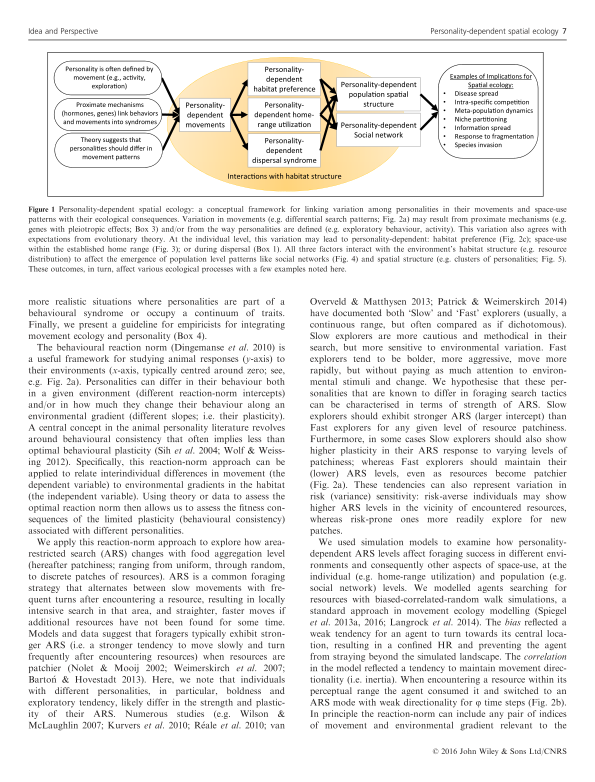
\includegraphics[width=0.7\linewidth]{fig01_spiegel_etal_2017.png}
    \caption{Spiegel et al. (2017) lay out a framework linking personality,
  movement, and resulting interactions. Personality may be initially
  measured in terms of movement, but the underlying causes can impact
  larger-scale processes such population spatial
  structure.}
    \label{fig:fig01_spiegel_etal_2017}
\end{figure}

\section{Modelling movement}

Many aspects of personality and movement can be explored using the waders \emph{Charadrii,} and especially the sandpipers Scolopacidae as a model system. Waders are a ubiquitous group of long-lived birds characterised by their littoral foraging on buried macrozoobenthic prey, and their often extreme flyway-channelled migration between generally disjointed and strongly seasonal global distributions \citep{boere2006a, gill2009, piersma2019}. Sandpipers are well known for their huge wintering fission-fusion flocks \citep{myers1983, conklin2008}, and as symbols of traditional landscapes \citep{colwell2018}. Waders (hereafter referring only to scolopacids) eking out their precarious existence at the waterline are thus poised to be the new canary in the coalmine: harbingers of global environmental change \citep{piersma2004, wikelski2016, fitzpatrick2018} which has swiftly advanced from `near' to `here' \citep{ipcc2018}. Wader movement fulfils many of the requirements one would expect from a system that integrates animal personality and movement studies. First, wader movement has been extensively investigated using a variety of approaches at nearly all spatio-temporal scales: small spatio-temporal scales such as foraging \citep{vangils2003, vangils2010}, large spatio-temporal scales such as migration \citep{buehler2006, piersma2011}, proximate causes for large-scale phenomena \citep{lank2003, ydenberg2004, ruthrauff2013, ruthrauff2018}, and ultimate causes for small-scale phenomena \citep{vangils2006, kraan2009}. Of the waders, red knots \emph{Calidris canutus} are among the best studied, with a wealth of biological information, from an understanding of physiology and its interaction with exploratory personality \citep{bijleveld2014, mathot2017}, to knowledge of group dynamics across scales \citep{bijleveld2010, bijleveld2012a, bijleveld2015b}, to the effect of foragers on their resource landscapes \citep{bijleveld2015c}.

Many theoretical studies increasingly employ agent-based approaches, which were developed to overcome two flaws in mathematical models \citep{huston1988}. First, in order to prevent an unreasonably large number of parameters (a disadvantage of ABMs), earlier models had abstracted populations to ``golden mean'' values that elided individual differences (see previous section) essential to evolutionary and ecological processes. The second issue was the assumption of global interactions, i.e., that all individuals affect all others equally, ignoring central problems of scale \citep{levin1992} and local interactions \citep[see][]{legendre1993} in ecology. ABMs have since been standardised in terminology \citep{grimm2006, grimm2010}, and are widespread in ecology \citep{deangelis2018}. In such models, individual organisms are each modelled separately and allowed to make decisions based upon various inputs, akin to real decision making processes \citep{deangelis2019}. In animal ecology, ABMs are especially relevant in modelling movement \citep[reviewed in][]{deangelis2005}, and have been used extensively \citep{spiegel2017, spiegel2013, getz2015, getz2016}, including to model red knots \citep{vangils2010}. Simple evolutionary algorithms \citep[see][]{back1996} as implemented in \citet{getz2015} and \citet{netz2017} that predicate the reproductive output (replicates) of each agent on some measure of fitness, such as net intake, can add eco-evolutionary dynamics to otherwise simple ABMs. This allows the modelling of movement across scales and contexts, from small-scale within-patch dynamics, such as competition \citep[see][ for a primer]{keddy2001} and the investigation of emergent large-scale evolutionary dynamics, such as community composition \citep[\emph{movement guilds};][]{getz2015}, and alternative strategies \citep{netz2017}. A major advance may be made by having the decisions of agents be the output of a `black-box' process in the form of artificial neural networks \citep[ANNs; see][ for example implementation]{lek1999, enquist2013, netz2017}. Neural network approaches allow for surprising results -- such as the evolution of rich movement dynamics and alternative strategies, even when beginning from largely similar populations \citep{netz2017, }.

\part{About this project}

In this section, I outline my approaches to examine the \textbf{\emph{evolution of movement types}} \citep[\emph{sensu}][]{wolf2010, getz2015} in the context of \textbf{\emph{environmental predictability and rate of change}} \citep[as in][]{botero2015}, using the \textbf{\emph{red knot system}} as a reference \citep{bijleveld2012a, bijleveld2014, bijleveld2015c, bijleveld2015b, oudman2016, oudman2018}. \citet{wolf2010} lay out the theoretical basis for the expectation that consistent behavioural differences could arise in spatially structured landscapes, while \citet{botero2015} describe how environments in certain regimes of temporal variability and predictability can give rise to similar polymorphisms. \citet{getz2015} and \citet{netz2017} show how virtual agents can evolve movement types while also structuring initially featureless landscapes. Bijleveld and colleagues (above) provide empirical data on the foraging and movement ecology of red knots that can inform modeling approaches and which may be used to test model predictions.

\section{Abstract models}

I will begin with an abstract approach and some basic questions. Modelling agent movement as the output of an ANN which takes environmental cues as outputs, I will first investigate how different regimes of landscape patchiness and temporal variability influence the evolution of movement types. Specifically, I will be interested in the following:

\begin{enumerate}
\def\labelenumi{\arabic{enumi}.}
\item
  \textbf{\emph{How many movement types are evolved under different regimes of spatial predictability and variability?}} This question is aimed at unifying the \citet{wolf2010} and \citet{botero2015} approaches at broad evolutionary scales. Recent mechanistic models based on ANNs suggest that genotype-phenotype mapping is not as clear-cut as in Botero and colleagues' work, and that polymorphisms (there identified as diversified hedged bets) may arise under a wider set of conditions in populations of fixed size. I will then examine the behaviour of agents (movement) in response to environment quality (resource landscape), with the idea being to identify the conditions under which different strategies (bet-hedging, plasticity, etc.) evolve.
\item
  \textbf{\emph{What is the link between behaviour and labile physiological state?}} Drawing inspiration from recent work in the red knot system that suggests a strong role for behaviour-sociality-physiology feedbacks \citetext{\citealp{bijleveld2014}; \citealp{mathot2017}; \citealp{oudman2016}; \citealp[discussed in][]{wolf2010}}, this question is aimed at investigating whether physiology constrains agents in behavioural parameter space. For example, when movement is made dependent on instantaneous state, it may be constrained by energy reserves, leading to a state-behaviour feedback. Further, intake may face digestive constraints that can strongly affect behaviour \citep{vangils2004}. I will investigate whether these feedbacks can produce behaviour-physiology clustering previously proposed in this system \citep{bijleveld2015b}.
\item
  \textbf{\emph{How do movement type frequencies develop over ecological and evolutionary time-scales?}} Foragers moving about a resource landscape can modify or introduce spatial patterns over time \citep{dejager2011, getz2015, netz2017}, yet effects such as facilitation remain understudied. Empirical results suggest top-down landscape structuring, such as by depletion, can be rapid \citep{bijleveld2015c}. Starting with initially unstructured landscapes, I will investigate how structure is modified using a relaxed version of \textbf{(1)} in which agents deplete their landscape at different rates. A natural consequences might be that foragers specialised to particular regimes of landscape structure could see a change in their profitability multiple times within their lives. When \textbf{(1)} includes the depletion element of \textbf{(3)}, agents might be expected to evolve a median (bet-hedged) phenotype that ensures profitability across landscape structures. This question is then aimed at investigating both the landscapes and agents:

  \begin{enumerate}
  \def\labelenumii{\alph{enumii}.}
  \item
    \textbf{\emph{How does landscape structure change over ecological and evolutionary time?}} In this scenario, I fall back upon the red knot system as a guide, that foragers are not always present on the landscape and the resource has time to regenerate. Such seasonal systems are widespread making this a reasonable scenario. I will investigate the development of landscape parameters over ecological and evolutionary time \citep[such as the autocorrelation range, or patch size; see][]{legendre1993} when agents are themselves evolving upon such landscapes.
  \item
    \textbf{\emph{How does the number and phenotype of movement types change over evolutionary time?}} Agents' consumption rates (set to be identical) could lead to different rates of landscape change in the scenario outlined above. Foragers would then evolve to maximise fitness in both space and time. As landscapes traverse the axis of patch size (autocorrelation range, or predictability) due to agent foraging, the spatial conditions that evolved types in \textbf{(1)} might recur multiple times. This should allow the investigation of whether there is a change in selection pressures on movement types, the time-scale at which it occurs, and whetfira codeher it is mediated by agents' effect on the landscape.
  \item
    \textbf{\emph{Do critical transitions occur in the number or profitability of movement types?}} As agent populations evolve movement types rather than bet-hedged phenotypes, these types may yet show sufficient flexibility to behaviourally buffer against decreasing profitability as the landscape shifts to a regime to which they are poorly adapted. This change may occur within individuals at ecological scales (as resources deplete or change over a season), and at the population level (as landscapes change over evolutionary time). Such systems, where the response (here, movement, or fitness) is initially poorly responsive to the driver (landscape structure, such as patch size), may then undergo abrupt transitions \citep{scheffer2009} to an alternative stable state. Behavioural changes relating to movement strategy occur in wader systems \citep{oudman2018}, but the process is not fully understood. I will look into whether changes in such systems can then be characterised as critical transitions. The same approach can be applied to the landscape, to study whether landscapes catastrophically shift to another state \citep[as in][]{vandekoppel1997, jefferies2006}.
  \end{enumerate}
\end{enumerate}

\section{Wader models and data}

Following the steps above, I will modify the models to simulate the red knot system. Important conceptual changes include the addition of regular environmental change in the form of the tidal cycle. This feature first limits resource landscape availability to agents. Second, it forces agent movement, further constraining the range within which agent movement types can specialise. For example, a very efficient movement type in a model elaborated above \textbf{(1)} would be to remain largely sedentary. This is not an option in tidal systems as most waders cannot swim. Important practical changes will be the parameterisation of the model following empirical data or best estimates on resource landscape structure and red knot physiology (body size, energy requirements, perception range).

Finally, I will turn to the empirical red knot tracking data and the benthic sampling data to investigate whether the models sketched above correspond to reality. The following questions suggest themselves.

\begin{enumerate}
\def\labelenumi{\arabic{enumi}.}
\setcounter{enumi}{3}
\item
  \textbf{\emph{Do red knots show movement types that can be identified
  from a combination of data sources?}} This question entails
  cooperation with my co-PhD student. Using scores from behavioural
  assays, state variables such as gizzard mass or body mass, and
  movement variables such as patch-switching or residence time, I will
  aim to determine whether knots evolved in models occupy comparable
  parameter spaces to real birds.
\item
  \textbf{\emph{Do red knots show assortative association based on
  movement type?}} Here, I investigate expectations from
  \citet{spiegel2017}, that association and the strength of social
  networks is strongly influenced by personality and the `clumped-ness'
  of the landscape. This question is suitable to both an experimental
  and field tracking approach.
\end{enumerate}

\part{Towards mechanistic movement models}

In each of these sub-sections, \textbf{\emph{Modelling landscapes}} and \textbf{\emph{Modelling agents}}, I will lay out how I propose to go about modelling the systems I have described above. I first describe the concept with some justification (usually drawn from red knot, or other avian systems), and then delve into the practical considerations of implementation, again seeking to justify my choices. In each case, I begin with the more abstract model, and then elaborate on a model based on red knots. It is important to note that while initial, abstract models are based on previous work, later, more complex models rely on these abstract models. Should the abstract models produce different dynamics from the ones expected from theory, the implementation and predictions of later models may have to be adjusted accordingly.

Another important point is that these are intended to be `mechanistic models of intermediate complexity'. For example, they will explicity model a mechanism of cue sensing, which was only implicitly assumed in \citet{botero2015}. Complexity, though significantly greater than Botero and colleagues' work, will have an upper limit set near that of \citet{netz2017} or \citet{vandenberg2015a}.

\section{Modelling landscapes}

\subsection{Concept: Spatial predictability}

Spatial pattern and scale matter in ecology \citep{levin1992}, and foragers benefit from responding to spatial structure in resource landscapes in empirical and theoretical studies \citep{benhamou1992, walsh1996, klaassen2006, vangils2006, vangils2010, oudman2018, bijleveld2016}. \citet{botero2015} model a very abstract predictability as well as variation in time -- however, space-time substitution \citet{blois2013} has found wide use in testing landscape-scale predictions in ecological systems \citep[e.g.][]{hirota2011, staver2011}, and allows the leveraging of extensive empirical sampling of resource landscapes at small \citep[e.g.][]{bijleveld2012} and large scales \citep[e.g.][]{huete2002}.

In a spatially structured landscape, autocorrelation is an important measure \citep{legendre1993}, and has been widely interpreted as corresponding to patch size \citep{kraan2009, kraan2009a, vangils2010, bijleveld2016, oudman2018}. This idea is easily illustrated by creating neutral landscapes with varying autocorrelation ranges -- landscapes with a high autocorrelation range have larger patches, and are more predictable (see Figure 3). In the wader-mudflat system, the mechanism underlying patch size does not need to be explicitly modelled to implement patch sizes. It suffices to understand that macrobenthic abundance is controlled by bottom-up processes over which agents have little influence.

\subsection{Concept: Temporal predictability and change}

The assumption of resources being independent of foraging agents is plainly ridiculous \citep{vandekoppel1997, jefferies2006, bijleveld2015c}. However, the proposed system is also far from agent-influenced resource generation \citep[see e.g.][]{leroux2018}. This leaves depletion as the main effect of agents on their landscape. Depletion then constitutes one important mechanism of temporal change in model landscapes. Agent-independent mechanisms such as seasonal growth and decline, or within-resource interactions (such as competition and facilitation) are the other major mechanism of temporal change in landscapes.

In initial models, agents will \emph{not} deplete the landscape. However, this would result in the trivial solution of agents remaining stationary at the first point where resources were above some threshold value. Models without depletion must then include some variation in the resource landscape such that agents are forced to move. This can be achieved by having the landscape change, either deterministically or stochastically \citep[see parellel with][]{botero2015}. The first approximates changes such as might be driven by seasonality, while the second is more akin to resource redistribution. The first approach allows near perfect prediction of resource values between times \emph{t} and \emph{t+1}. In the second case, if the `redistribution' is highly variable, i.e., values at a coordinate at a time \emph{t} have a wide range of correlation with values at time \emph{t+1}, temporal predictability is reduced. The two extreme cases allow the examination of the interacting effects of spatial and temporal predicatability, and identification of the more interesting regime for further investigation.

In a model tailored to waders, the situation is compounded by another source of temporal variation: the tidal cycle. This highly periodic phenomenon both gives and takes away: water restricts exploitation of parts of the landscape (most waders cannot swim; but see interesting exception of phalaropes \emph{Phalaropus}). However, the tide also allows waders to use their pressure-sensitive bills \citep{piersma1998} to find prey in the waterlogged substrate. This results in gradients of information on prey availability at different scales. At the landscape scale, the optimal prey search area is at the waterline where the substrate is exposed yet sufficiently wet to allow knots to probe for food. At smaller scales, this prey-sensing mechanism severely localises information on potential intake, i.e., a foraging wader can only directly assess the quality of its immediate neighbourhood. The dynamics of coastal systems cause further complications -- but also create opportunities -- when modelling agents, and these are discussed later.

\subsection{Practice: Modelling spatio-temporal change in landscapes}

Both resource and tidal landscapes may be implemented in continuous space. While implemented in some models \citep[e.g.][]{spiegel2013, spiegel2017}, continuous space creates a mismatch of resolution between simulations and empirical data, which is an important consideration in this project. Since data from benthic sampling can be converted into predicted intake rate rasters with a maximum resolution of 10 m \citetext{\citealp[see method in][]{bijleveld2012}; \citealp[examples in][]{oudman2018}}, the resource landscape is best modelled as a two-dimensional square grid of side \emph{n} cells, a common approach \citep{nolet2002, vangils2010, getz2015, netz2017}. Grid values can be modelled using flexible tools \citep{sciaini2018} as Gaussian random fields \citep{turner2015d, kery2019}. Working on the logic of infinite extent \citep{nolet2006}, the grid boundaries are periodic. Landscapes can thus easily be assigned an autocorrelation regime. Grid cells in this landscape are initialised with certain values of resource between 0.0 and 1.0. This allows the subsequent mapping of empirical values using a variety of functions, such as the sigmoidal \citep{gershenfeld1999}.

\begin{figure}

    \includegraphics[width=0.7\linewidth]{intro_essay_figure3.png}
    \caption{Examples of Gaussian random field neutral landscapes generated in R
  following methods from Sciaini et al. (2018). \textbf{(a)} Landscapes of side
  100 cells, with increasing autocorrelation range (numbers above panels).
  Larger autocorrelation ranges result in smoother transitions between
  areas of high (blue) and low (red) resources, and thus larger patches.
  \textbf{(b)} Spatial autocorrelation in simulated landscapes; each panel
  corresponds to the one directly above in \textbf{(a)}. Compare with figures
  in Oudman et al. (2018).}
    \label{fig:intro_essay_figure3}
\end{figure}

The tidal landscape's elevation is easily modelled as a distance or edge gradient \citep{etherington2015}. This creates a region of high elevation which is always exposed, approximating islands such as Griend where waders roost. This model will use a circular distance gradient that avoid issues arising from landscape edges. Temporal change in both water level and resource landscapes can initially be considered to be the output of a sine function with a wavelength \emph{R} \citep[as in][]{botero2015}: the ``relative timescale of environmental change'' of each. For water level, the wavelength would be the number of discrete model timesteps contained in one unit of ecological time. Since the tidal cycle (approx. 13 hours off Griend in 2017; \emph{unpublished data}) is a prominent feature, it is intuitive to also consider this a unit of ecological time, with a single non-breeding season comprising some 6 -- 8 months (approx. 450 tidal cycles). Each season would then be a unit of evolutionary time. In the case of the resource landscape, the wavelength can be set to vary across a range to mimic either seasonal (renewal each season) or long-term (climatic cycles) dynamics, corresponding very well to \citet{botero2015}.

\section{Modelling agents}

\subsection{Concept: Agent Based Models}

I will implement ABMs (see Section 2.3) first for abstract foragers, and second for foragers similar to waders. While waders are an ideal system in which to study foraging, they are specialised upon a small subset of resources and ecological conditions that will constrain more realistic models. For a general forager, it is important to be able to gain some key information: its position, the profitability of its position, and its potential future positions \citep[\emph{why} and \emph{where} to move;][]{nathan2008a}. An agent will move when its current location cannot sustain it, possibly due to some metabolic requirement \citep{barraquand2008}. There is a strong interplay between \emph{where} to move and \emph{how} to move when agents are capable of more than one movement mode, such as in birds which can switch from cursorial to volant. While the exact mechanism may be abstracted, movement carries a cost, and this cost must be taken into account when deciding when and where to move \citep{charnov1976a}. Movement decisions can be made as the result of explicitly written functions \citep[e.g.][]{getz2015}, but this entails and often elides implicit assumptions about the functional response of agents to their environment. This environment may include other agents, allowing for facilitation by local enhancement \citep{beauchamp2013}.

\subsection{Concept: Agent-resource and agent-agent interactions}

In the models sketched above I began with the assumption that while especially large or numerous foragers (ecosystem engineers) are capable of transforming their resource landscapes \citep{laundre2001, jefferies2006, leroux2018}, this cannot be expected for all consumer-resource systems. However, there is evidence from observational studies at small spatial scales (approx. 0.067 km\textsuperscript{2}) that medium-sized foragers can significantly deplete their resources \citep{guillemette1996, jefferies2006}. Markedly smaller waders too can deplete resources over small spatio-temporal scales \citep{szekely1992, vangils2003, bijleveld2015c}. Thus, in more realistic models, I will allow foragers to deplete their landscapes. This depletion will replace the sinusoidal temporal variation I proposed for initial abstract models, and will more realistically approximate seasonal dynamics where resource replenishment occurs in a single growing period, and further declines are largely due to harvesting.

Depletion indtroduces the prospect of exploitative competition \citep{keddy2001}, where agents affect each other by consuming shared resources. Its inclusion in the simplest models has stark eco-evolutionary consequences -- for example, \citet{getz2015} showed that larger population sizes (and thus higher competition) resulted in more movement types and a more rapid rate of evolution. I propose to take this into account by on a grid cell proportional to the number of agents on the cell. Interference competition is widely seen in waders \citep{goss-custard1980}, yet is also more challenging to include in discrete time models \citep{vahl2006}. I will leave this aspect of wader ecology out of the model (but see next sub-section).

\subsection{Concept: Modelling interference competition}

I intend to co-supervise a master's student with an interest in evolutionary game theory, and modelling skills. This master's project will extend the work of \citet{vahl2006}, and take into account the following: first, that mechanisms can strongly influence the dynamics of games \citep{vandenberg2015a}, second, that competition is often state dependent \citep{vangils2004}, and third, that both direct and indirect competition \citep{vahl2005, bijleveld2012a} can have consequences for agent space-use \citep{vahl2007a}. I envision the following modules for this project: individual based models following Vahl's ideas, with pairwise interactions determining some contest outcome that translates to fitness. These will be implemented in an evolutionary system, where successful agents replicate, either with fixed or flexible population size. Second, some state dependence of behaviour to examine behaviour -- physiology trade-offs. Third, to have the agent decisions be the output of neural networks. Fourth, implementation in an initially limited spatial system (with the option of expansion), such as a two dimensional 3 × 3 grid, or a single dimensional vector. In this final, more realistic system, movement would be an option, allowing interesting dynamics between direct competition, state-dependence of behaviour, and spatial distribution in a game theoretical framework.

\subsection{Practice: Agent Based Models using Artificial Neural Networks}

Agents in ABMs possess attributes, including knowledge of their coordinate position on the grid (\emph{x, y}) and some proxy of internal state \citep[energy reserves; e.g.][]{vangils2010}. Other attributes may comprise the overall phenotype of the agent. For example, \citet{getz2015}; \citet{getz2016} draw three parameters that correspond broadly to giving-up value $\rho$, competitiveness $\delta$, and sociability $\alpha$ from suitable distributions, and assign them to agents. These values are implastic through the agent's life, and while a useful starting point, assumes behavioural consistency. The ANN approach allows for far richer dynamics, where agents assess their environment (described above) and make a single decision about what move to make in the next time-step. This environment may include landscape values and/or other agents \citep{netz2017}. These cues are the activations of the agent's ANN nodes, while state variables can be mapped to node weights and biases. Agent movement is often limited to the Moore neighbourhood of size 1, i.e., from agent grid position to the eight cells around it in each timestep \citep{getz2015, netz2017}. Movements of unit distance in unit time assume constant speed; clearly unfounded since real animals such as knots can achieve at least two broad movement speeds by flying or walking (Bijleveld et al. \emph{unpublished data}). The ANN output sketched above -- next grid position -- allows agents to choose their movement distance at each time step. At an ecological scale, this first allows the investigation of individual consistency in step length, and then an examination of whether movement types have characteristic step lengths, e.g.~that are some whole number multiple of the autocorrelation range. Movement carries a travel cost, which is subtracted from energy reserves at each time-step.

In more complex models, cues of where best to forage need not be equally available to foraging agents. Knots can sense only very local macrobenthos availability using their pressure sensitive bills \citep{piersma1998}. At intermediate and local scales, knots may use public information from other foragers \citep{bijleveld2015b}, while it is to be assumed that across scales, knots are able to avoid deep water. This creates a cue gradient: at very small range, agents have much more reliable information than at larger ones, where local enhancement due to conspecific presence may play a greater role \citep{beauchamp2013}. Thus agents in such models may evolve movement types that trade the cost of poor information for the cost of exploitative competition, and vice-versa, all while balancing the cost of travel with the intake from the landscape. Evolutionary models require that traits are inherited, implying reproduction, birth and death. Agent fitness is best modelled as some function, possibly sigmoidal, of net intake, i.e., agents do have an upper limit to the offspring produced; for example, many sandpipers produce a clutch of four eggs \citep{piersma2019}, and this is a realistic upper limit. Agents must therefore also have some mechanism approximating death; this can be modelled as energy reserves reaching zero, after which the agent dies. Agents must reproduce at some time --- in systems worldwide, most species have a fixed breeding season, and this can be modelled as agents that survive until the next ecological time-step producing offspring. The value of energy reserves at which agents decide to reproduce may also be allowed to evolve, possibly evolving interesting life-history strategies \citep[as in][]{wolf2012, wolf2007a}.

\section{Confronting models with data}

Models are always wrong, but they do yield insights into real systems. Empirical data on the red knot system is collected both from the agents \citetext{\citealp[ in \citet{bijleveld2015b}]{maccurdy2015}; \citealp[examples in][]{bijleveld2016}; \citealp{oudman2018}} and their resource lanscape \citep{bijleveld2012}. These data include morphometic measures, as well as movement measures which may be obtained using a number of tools now available for the processing of animal tracking data \citep[most recent review by][]{joo2019}. Coupled with behavioural scores from aviary experiments \citep[currently ongoing at NIOZ; see e.g.][]{bijleveld2012a, bijleveld2015b}, these can be used to cluster individuals. These clusters can then be compared with movement types evolved in simulations. I aim to given the resource landscape structure experienced in the Wadden Sea by \emph{islandica} red knots, and then to examine how well these predictions hold up in the face of data.

Individual associations of red knots are not expected to be non-random, consistent with the pattern for other waders \citep{myers1983, conklin2008}. However, that expectation might yet hold for movement types rather than specific individuals, with assortative association within or between types in different environmental regimes \citep{spiegel2017}. The strength and nature of associations can be quantified from simulated movement tracks, and then tested using extensive tracking data.

\newpage

\newgeometry{bottom=10mm}

\part{Timeframe}

This is an approximate timeframe. Events farther in the future are more likely to change. Note that field visits and review meetings are not included, and that flexible plans are marked by asterisks.

%\nolinenumbers

\begin{table}
\begin{turn}{90}
\begin{tabular}{llllll}
\toprule
{\footnotesize{}Id} & \textbf{\footnotesize{}Year} & \textbf{\footnotesize{}Research} & \textbf{\footnotesize{}Training/conferences} & \textbf{\footnotesize{}Co-supervision} & \textbf{\footnotesize{}Output}\tabularnewline
\toprule

 & \textbf{\footnotesize{}2018} & \textbf{\footnotesize{}First 9 months} &  &  & \tabularnewline
\hline
{\footnotesize{}1} & {\footnotesize{}May -- Jun} &  & {\footnotesize{}Visit NIOZ} &  & \tabularnewline
\hdashline
{\footnotesize{}2} & {\footnotesize{}Jul \textendash{} Sep} & {\footnotesize{}Field visits; knot associations} & {\footnotesize{}Computing cluster crs.; \emph{Biomove symp.}} &  & {\footnotesize{}Poster Biomove symp.}\tabularnewline
\hdashline
{\footnotesize{}3} & {\footnotesize{}Oct \textendash{} Dec} & {\footnotesize{}Lit. rev. for intro. essay} & {\footnotesize{}\emph{C++ programming; PhD course CRI}} & {\footnotesize{}B.Sc. essays (2)} & {\footnotesize{}Crs. proj. (2); Intro. Essay}\tabularnewline

\toprule
 & \textbf{\footnotesize{}2019} & \textbf{\footnotesize{}Building abstract models} &  &  & \tabularnewline
\hline
{\footnotesize{}4} & {\footnotesize{}Jan \textendash{} Mar} & {\footnotesize{}Move. + competition model descriptions} & {\footnotesize{}GRS/GRC; \emph{Sci. Integrity Course}} & {\footnotesize{}M.Sc. student 1, 2} & {\footnotesize{}Final Intro. Essay}\tabularnewline
\hdashline
{\footnotesize{}5} & {\footnotesize{}Apr \textendash{} Jun} & {\footnotesize{}\makecell[l]{Proj. 1. Movement mods. variable envmnt.; \\ Proj. 2. Interference mods.}} & {\footnotesize{}Visit NIOZ} & {\footnotesize{}MSc student 1, 2} & {\footnotesize{}Proj. 1+2. methods}\tabularnewline
\hdashline
{\footnotesize{}6} & {\footnotesize{}Jul \textendash{} Sep} & {\footnotesize{}Proj. 3. Aviary scores \textasciitilde{} field movement} & {\footnotesize{}Collaborators visit{*}} & {\footnotesize{}MSc student 2} & {\footnotesize{}Prep. Proj. 3. m/s.}\tabularnewline
\hdashline
{\footnotesize{}7} & {\footnotesize{}Oct \textendash{} Dec} & {\footnotesize{}Analyse data Proj. 1+2.} & {\footnotesize{}Machine learning course{*}} &  & {\footnotesize{}Proj. 3 m/s.}\tabularnewline

\toprule
 & \textbf{\footnotesize{}2020} & \textbf{\footnotesize{}Building shorebird models} &  &  & \tabularnewline
\hline
{\footnotesize{}8} & {\footnotesize{}Jan \textendash{} Mar} & {\footnotesize{}Proj. 4. Develop shorebird models} & {\footnotesize{}\emph{Modelling in R} course;} & {\footnotesize{}MSc student 3, 4{*}} & {\footnotesize{}Proj. 1+2 m/s.}\tabularnewline
\hdashline
{\footnotesize{}9} & {\footnotesize{}Apr \textendash{} Jun} & {\footnotesize{}Finalise shorebird models} & {\footnotesize{}Collaborators visit*} & {\footnotesize{}MSc student 3, 4{*}} & {\footnotesize{}Shorebird mods. methods}\tabularnewline
\hdashline
{\footnotesize{}10} & {\footnotesize{}Jul \textendash{} Sep} & {\footnotesize{}Proj. 5. MSc students' project topics} & {\footnotesize{}ISBE/ESEB} & {\footnotesize{}MSc student 3, 4{*}} & \tabularnewline
\hdashline
{\footnotesize{}11} & {\footnotesize{}Oct \textendash{} Dec} & {\footnotesize{}Compare models with data} &  &  & \tabularnewline

\toprule
 & \textbf{\footnotesize{}2021} & \textbf{\footnotesize{}Drawing down} &  &  & \tabularnewline
\hline
{\footnotesize{}12} & {\footnotesize{}Jan \textendash{} Mar} & {\footnotesize{}Compare models and data} &  &  & {\footnotesize{}Proj. 4+5 m/s prep.}\tabularnewline
\hdashline
{\footnotesize{}13} & {\footnotesize{}Apr \textendash{} Jun} & {\footnotesize{}Paper writing} & {\footnotesize{}Visit collaborator/future lab{*}} &  & {\footnotesize{}Proj. 4+5 m/s}\tabularnewline
\hdashline
{\footnotesize{}14} & {\footnotesize{}Jul \textendash{} Sep} & {\footnotesize{}Paper writing} &  &  & \tabularnewline
\hdashline
{\footnotesize{}15} & {\footnotesize{}Oct \textendash{} Dec} & {\footnotesize{}Thesis and paper writing} & {\footnotesize{}GSSE \emph{Career Perspectives Courses}} &  & \tabularnewline

\toprule
 & \textbf{\footnotesize{}2022} & \textbf{\footnotesize{}Preparing to leave} &  &  & \tabularnewline
\hline
{\footnotesize{}16} & {\footnotesize{}Jan \textendash{} Mar} & {\footnotesize{}Thesis and paper writing} & {\footnotesize{}Post-doc grant writing} &  & {\footnotesize{}Post-doc grant appl.}\tabularnewline
\hdashline
{\footnotesize{}17} & {\footnotesize{}Apr \textendash{} May} & {\footnotesize{}PhD ends; thesis submission} &  &  & {\footnotesize{}PhD thesis}\tabularnewline
\hdashline
{\footnotesize{}18} & {\footnotesize{} Sep} & {\footnotesize{}Preparation \& PhD defence} &  &  & \tabularnewline

\bottomrule

\end{tabular}
\end{turn}

\caption{}

\end{table}

\newpage

\restoregeometry

\part{References}
\footnotesize
%\changemargin{-1.0cm}{-1.0cm}

\setstretch{1.0}
\setlength{\parskip}{3pt plus 2pt minus 1pt}
\setlength{\parindent}{-3ex}
\indent
\bibliography{citationLibPrg2019.bib}

\end{document}
